\section{Chapter Overview}

In the System Evaluation chapter we will touch on the overall design of the system while also comparing it to the project objectives that were stated in the Introduction chapter 2.9, the testing that went into the project will also be documented. We will finish off by reviewing any limitations and areas of improvement in the project 

\section{Project objectives}

Initially we set out to create a universal web-based restaurant management and point-of-sale system that could be used on any premises that require a till system to process payments, print receipts, use a bar-code scanner as well as being able to generate reports. We felt that with the final product now complete we have achieved this goal as our web application is capable of all of the above, we feel it would be a great help to any site that needed a restaurant management and point-of-sale system. Other objectives included:

\begin{itemize}
  \item User Authentication
  \item Till GUI
  \item Sales
  \item Receipts/Hardware
  \item Reports
  \item Users
  \item Categories
  \item Products
  
\end{itemize}

\section{Testing}

We felt that it was of utmost importance to fully test our web application in the development as well as in the completion of the project. Some of the testing we conducted included Graphical User Interface(GUI) testing, Functional testing, Unit Testing and finally End to End testing.

\subsection{GUI testing}

GUI testing is a software testing type in which tests the Graphical User Interface of the Project, This involves checking the screens with controls such as sidebar menus, buttons, icons , dialog boxes etc. The goal of GUI Testing is to make sure the UI works as designed.
\newline
\newline
We decided to simply check some buttons and sidebar menu options in our bid to test the GUI functionality. In the following figure we show how the "Products" sidebar menu option leads to the products page then we test that the "Add Product" button works as designed.
\newline
\newline


\begin{figure}[h!]
	\caption{GUI Testing.}
	\label{image:myImageName}
	\centering
	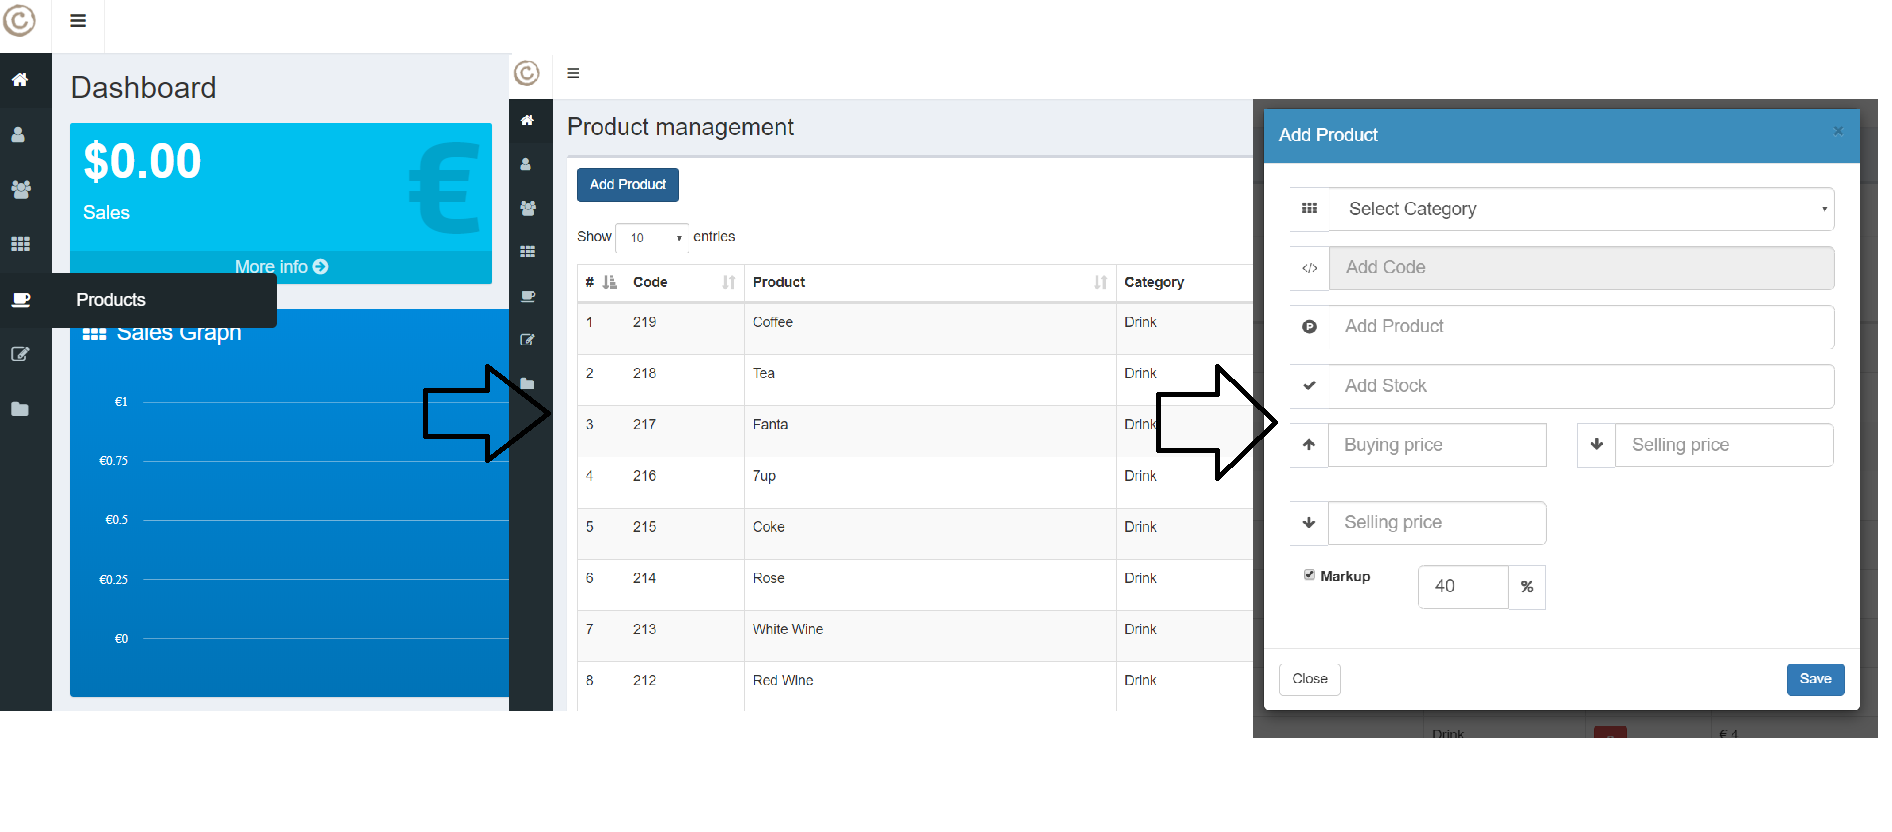
\includegraphics[width=0.9\textwidth]{Fig images/guitesting1+2+3.png}
\end{figure}

As you can see both the menu option as well as the button work as designed as the Product options brings the user to the Products page while the Add products button directs the user to the creation of a new product.

\subsection{Functional Testing}

Functional testing is a type of software testing where you test the software system against the functional requirements.  The purpose of one of these tests is to determine that the when inputting data into some parts of the software application the correct output is shown.
\newline
\newline
For our functional test we decided to stick with testing our products, once the add products button was clicked we moved onto inputting data to add a brand new product to verify that the functionality of add product was working as expected.
\newline
\newline


\begin{figure}[h!]
	\caption{Functional Testing.}
	\label{image:myImageName}
	\centering
	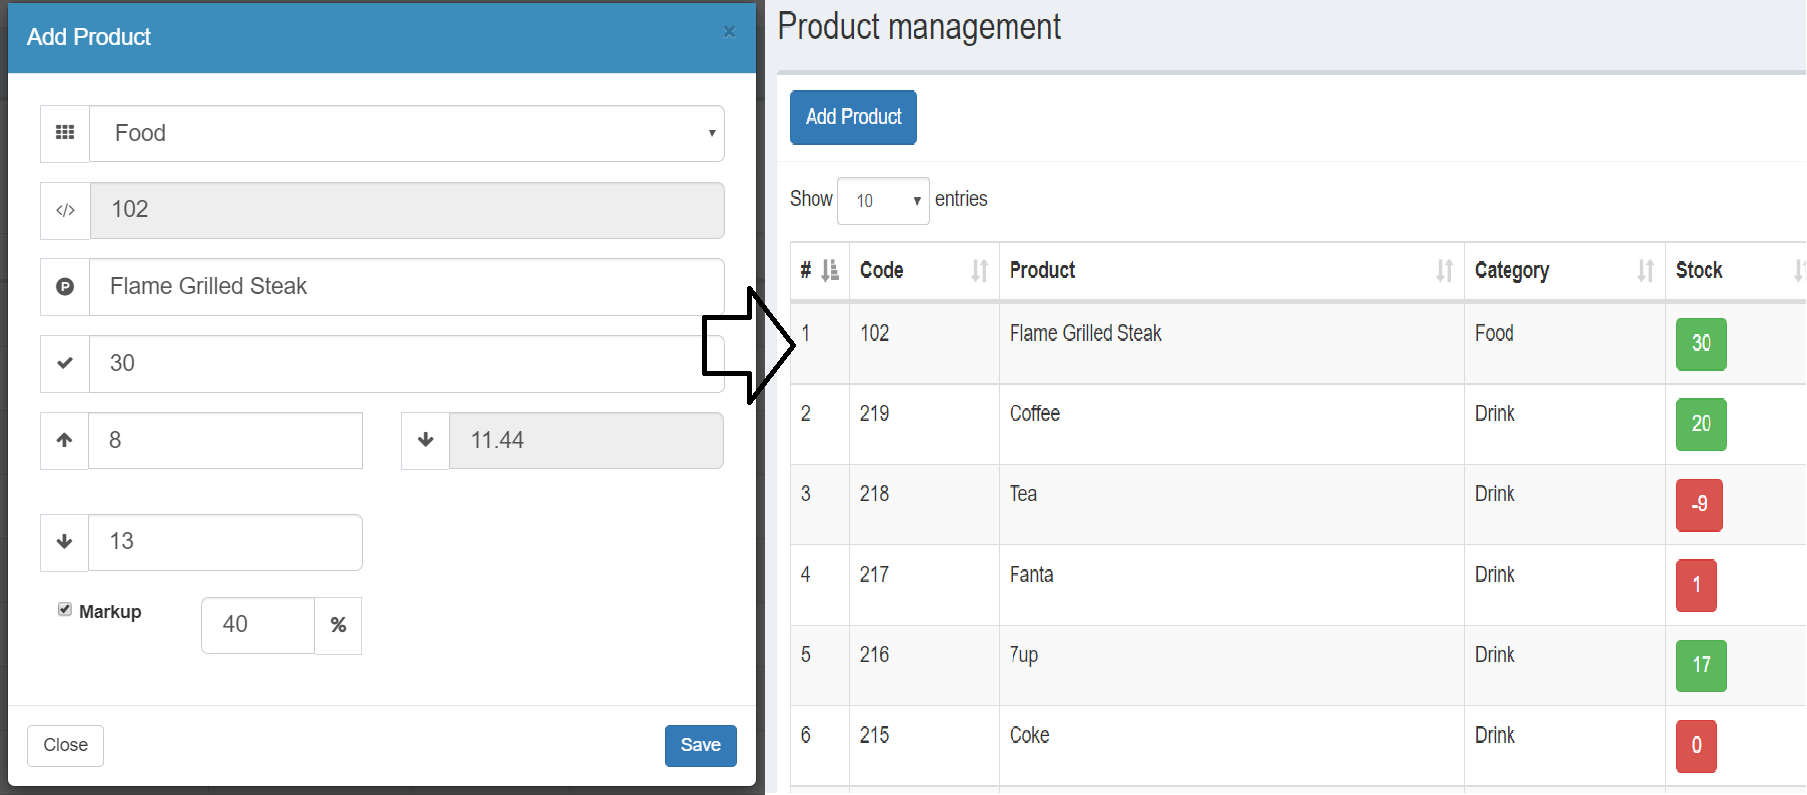
\includegraphics[width=0.9\textwidth]{Fig images/Functionaltest1+2.png}
\end{figure}


As displayed in the figure above you can see that once the user has input all the data needed for the creation of a product and clicks create product, the system will then system will then redirect the user to the products page with the newly created product displayed at the top of the Products table.

\subsection{Unit Testing}
Unit testing is the testing of individual units or components of a software. The reason that it is done this way is to validate that each unit of the software code performs as expected.
\newline
\newline
In our bid to do some unit test we decided to test the code that correlates to adding products to the database table.
\newline
\newline


\begin{figure}[h!]
	\caption{Unit Testing.}
	\label{image:myImageName}
	\centering
	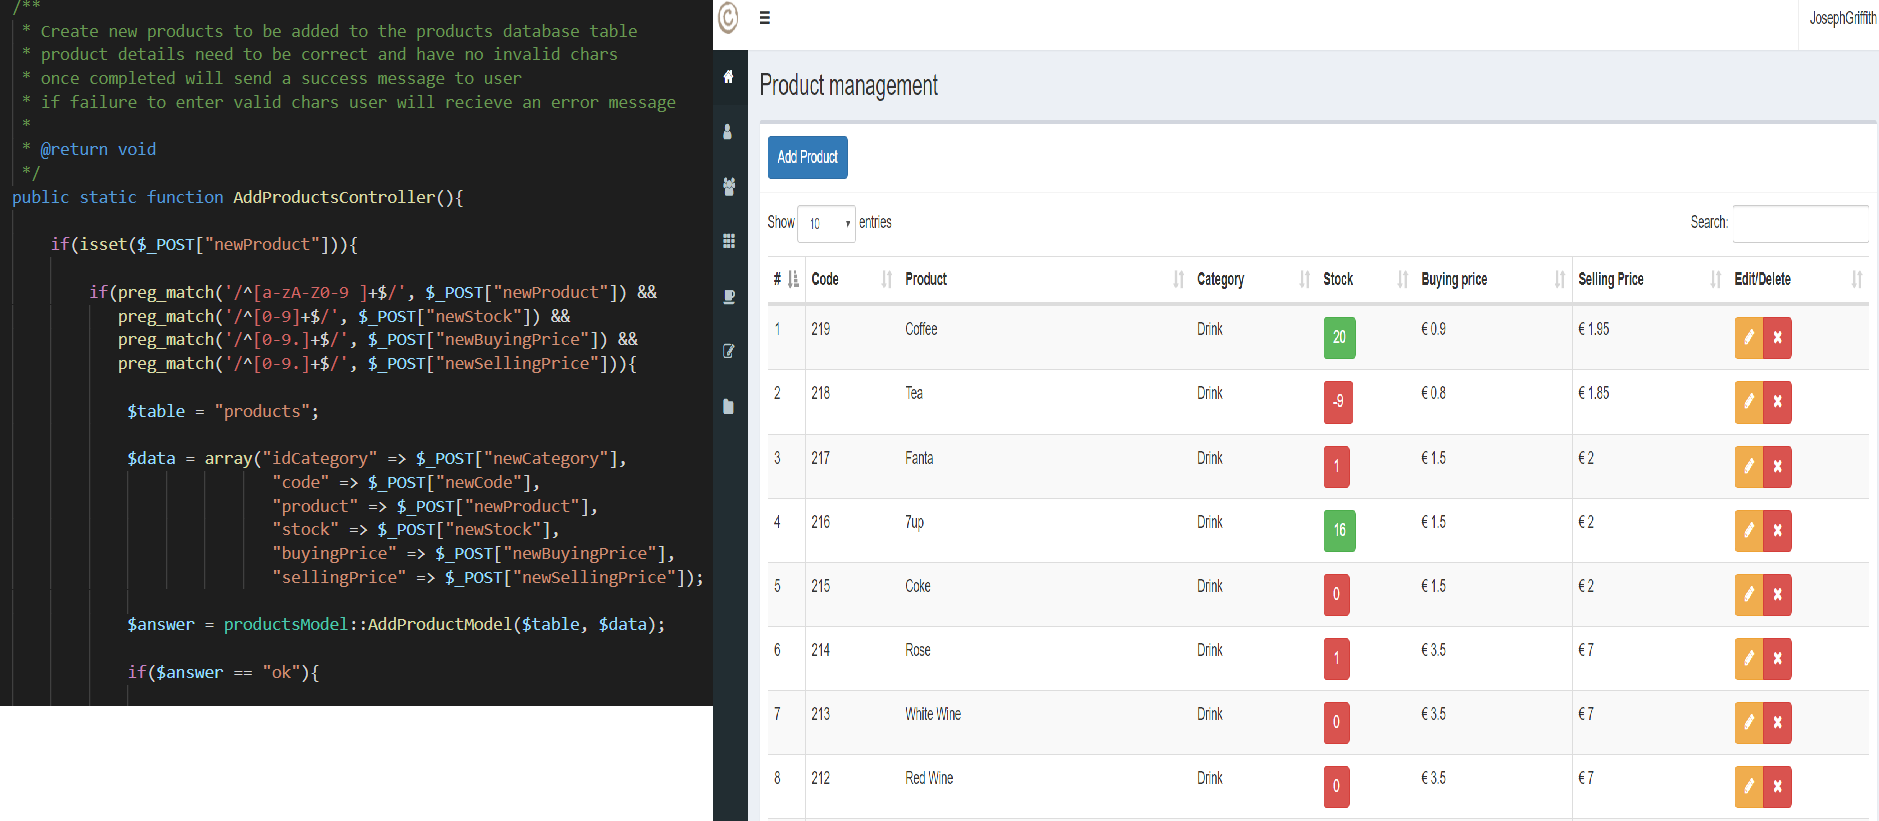
\includegraphics[width=0.9\textwidth]{Fig images/Unittest1+gui3.png}
\end{figure}


As shown above the code snippet which is in charge of fetching and displaying the creation of the desired product and table displayed is working as intended.

\subsection{End to End Testing}
End to End testing is a type of software testing where the tester validates the software system along with its integration with external interfaces. The purpose to this specific testing is to test a production like scenario
\newline
\newline
In the end to end testing we just decided to go through logging in, creating a sale, printing a receipt then finally logging back out.
\newline
\newline


\begin{figure}[h!]
	\caption{End to End Testing.}
	\label{image:myImageName}
	\centering
	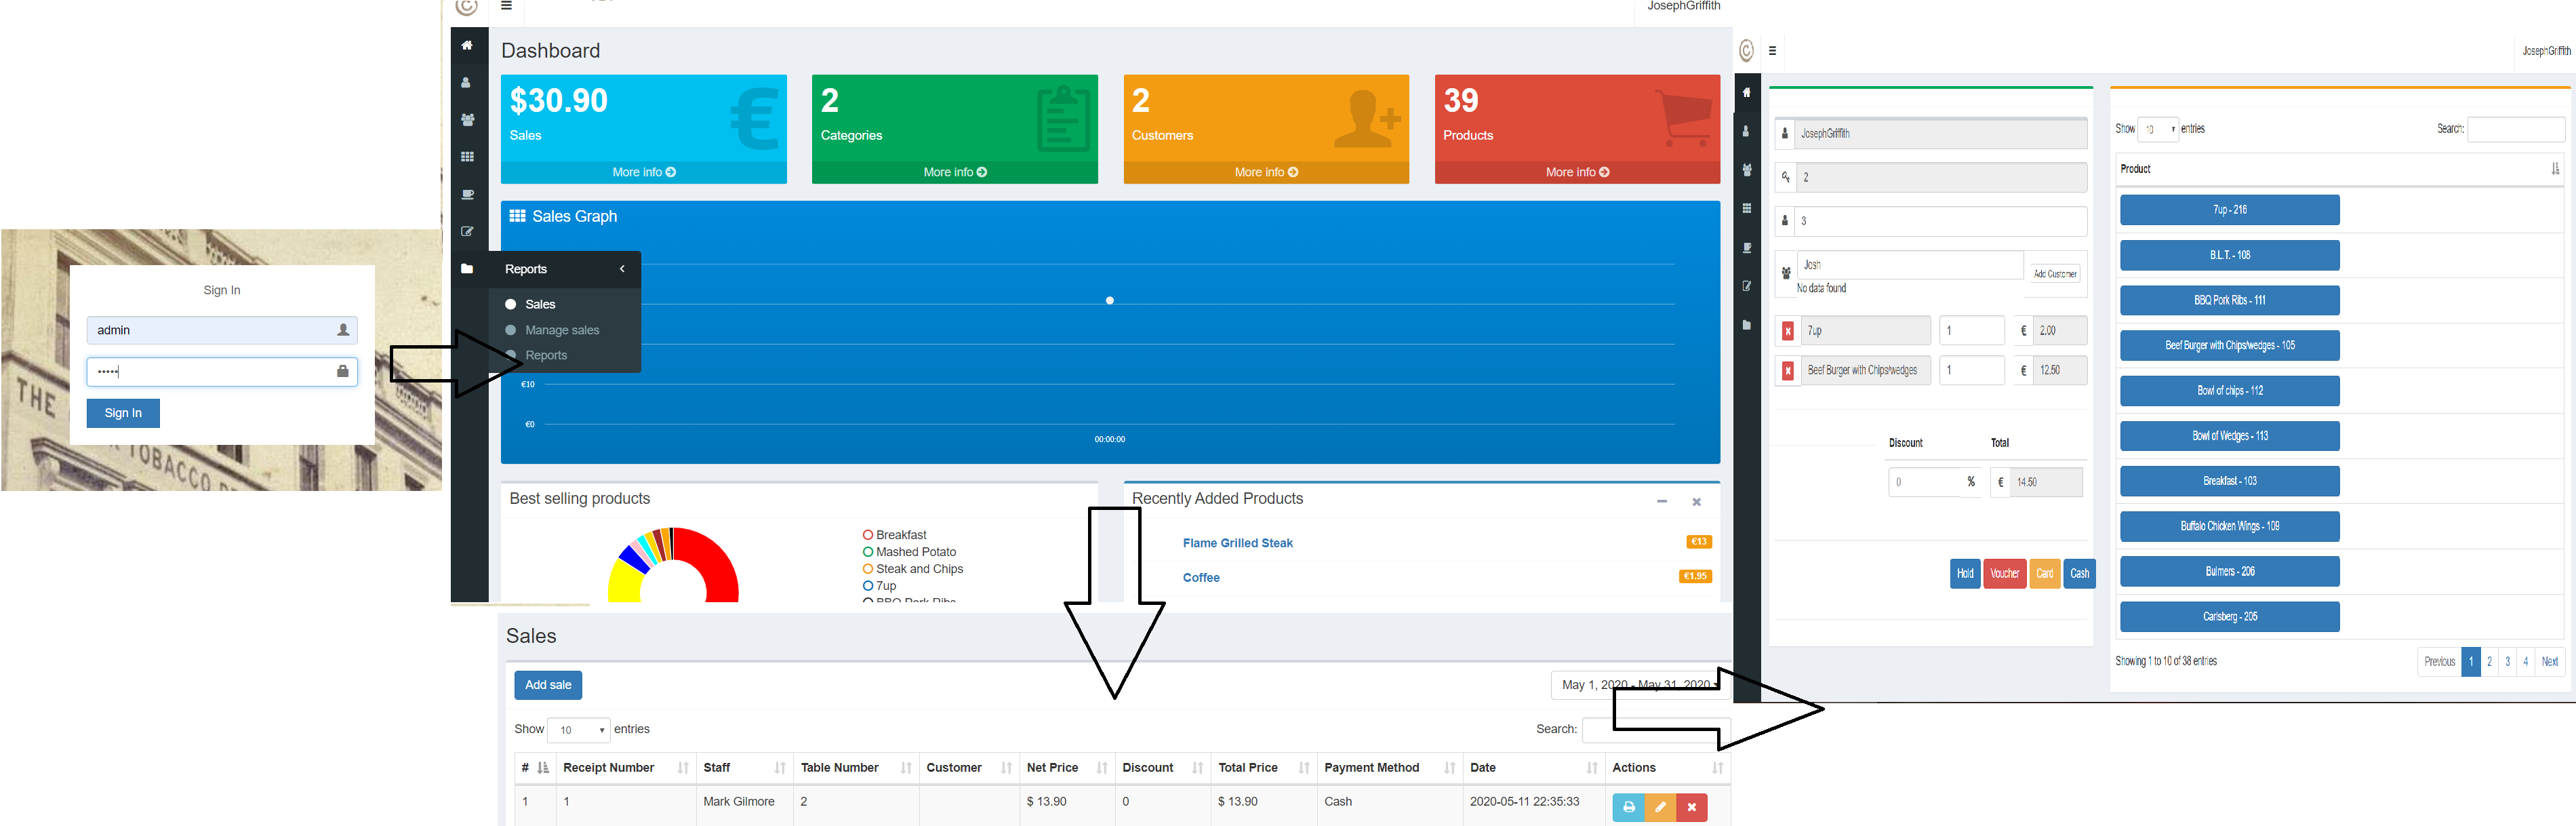
\includegraphics[width=0.9\textwidth]{Fig images/endTOend1-5.png}
\end{figure}
\begin{figure}[h!]
	\caption{End to End Testing. pt2}
	\label{image:myImageName}
	\centering
	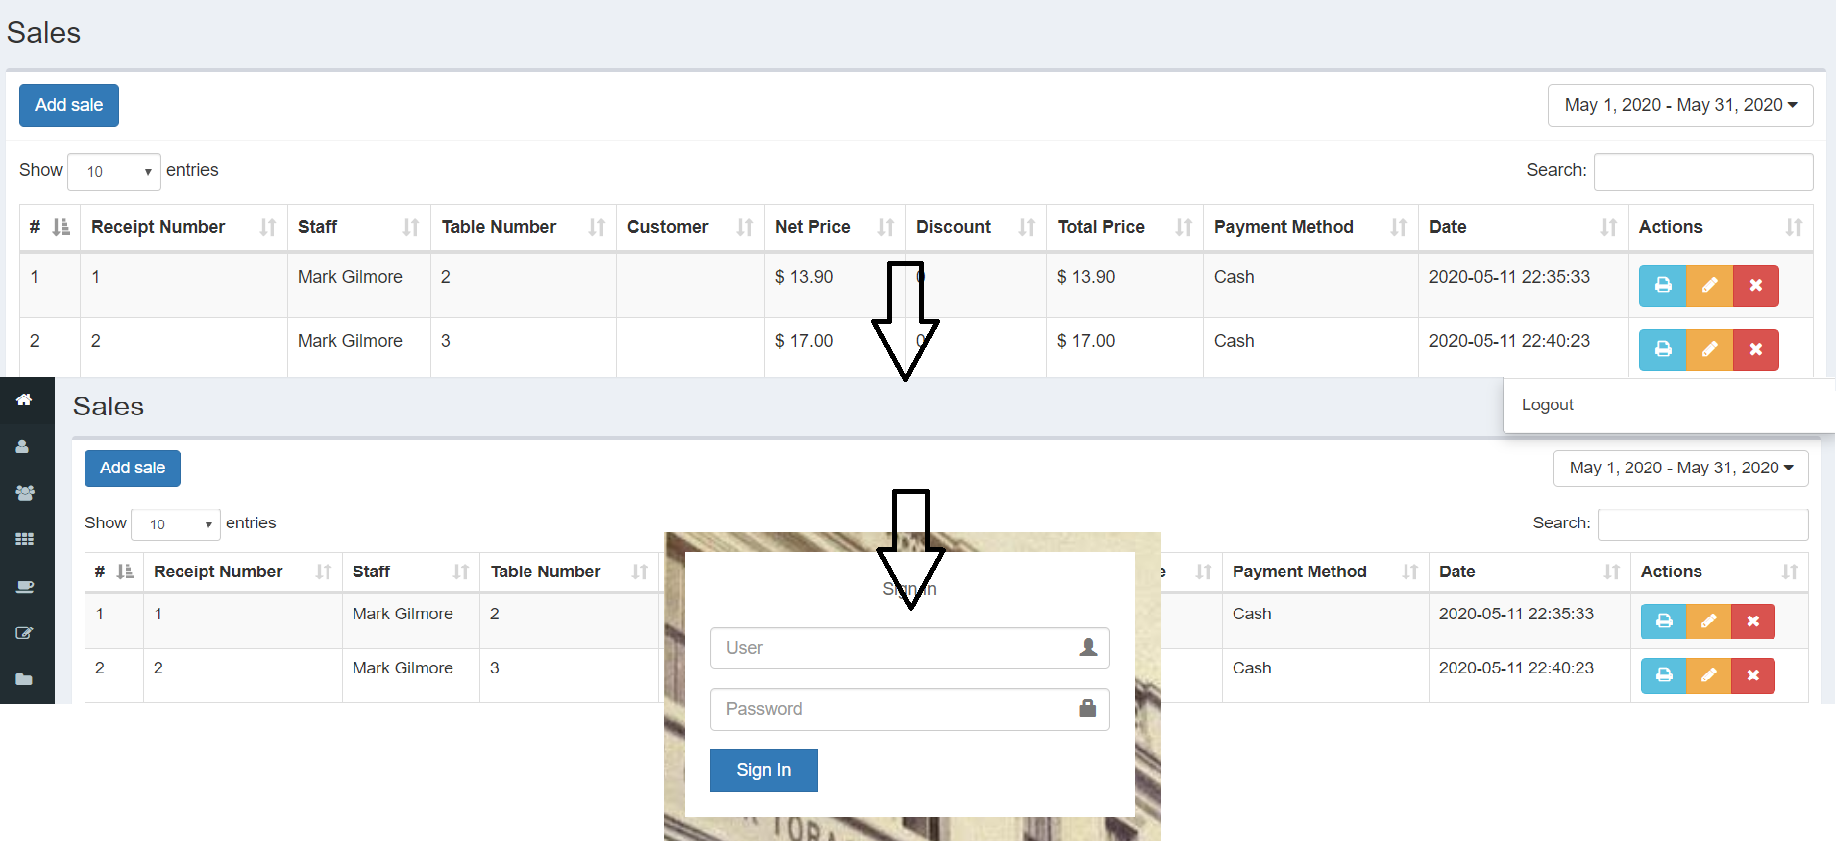
\includegraphics[width=0.9\textwidth]{Fig images/endTOend6-8.png}
\end{figure}


As expected the system works as intended where the user can log into the system then create a sale, print the receipt for the sale then finally log out of the system.


\section{Limitations and areas of Improvement in the project}

\subsection{Limitations}

As of now the biggest limitation we are facing is not having the web application on the cloud this proves as a major set back as it is essential for us to have the application up and running on the cloud so that any businesses in the future would want to sample our software.

\subsection{Improvements}

Improvements that can be made to the current system could include adding a remote receipt printer, creating a loyalty system such as a loyalty code for returning customers where the customer would receive discounts for continued purchases or add item sales where some items on the menu would be on sale at different dates for example early birds deal where the customer gets a small discount on breakfast early in the morning.
